\chapter{View Synthesis Generation}
\label{chap:chap_05}
\vspace{-8mm}

In chapter~\ref{chap:chap_02} we discussed how to approach scene reconstruction using classical and CNN based methods. We first reviewed specific parts of the pipeline that uses local features to detect and describe regions of interest later used to perform the 3d reconstruction. Having a pipeline where you can switch and replace some components eases those cases where you want to parallelize processes, detect errors or even perform offline optimisation of those specific parts. However, as we remarked in chapter 3, the trend for deep learning is to design the entire pipeline in an end to end fashion and optimise all the components of the pipeline under the same optimisation framework. For this reason, we introduced Kornia a framework that provides a wide variety of tools to combine classical vision with deep neural networks. In this chapter we are going focus on the design of a system to perform scene reconstruction trained following the mentioned end-to-end trend, and combining classical computer vision functions of projective geometry inside the system computational graph.

In the next sections we present a novel approach for synthesizing realistic depth maps of deformable clothes from arbitrary views. Given a depth map of a hanging cloth captured from a camera, our model renders the depth map of how this cloth would be seen under a new camera pose, realistically hallucinating the occluded parts and their most likely creases and folds. While view synthesis is a well known problem in the RGB domain, it is still quite unexplored for inferring novel geometry, and specially for highly deformable objects. In this scenario the problem becomes specially challenging due to the large amount of ambiguities and possible shapes. In order to tackle this  problem we propose a novel architecture that performs geometry and occlusion reasoning in the feature space and combines it with adversarial learning. Extensive evaluation shows that our approach, while being relatively simple, is able to generate novel views of complex cloth configurations in both simulated and real scenarios. 

\newpage

\begin{figure*}
\begin{center}
    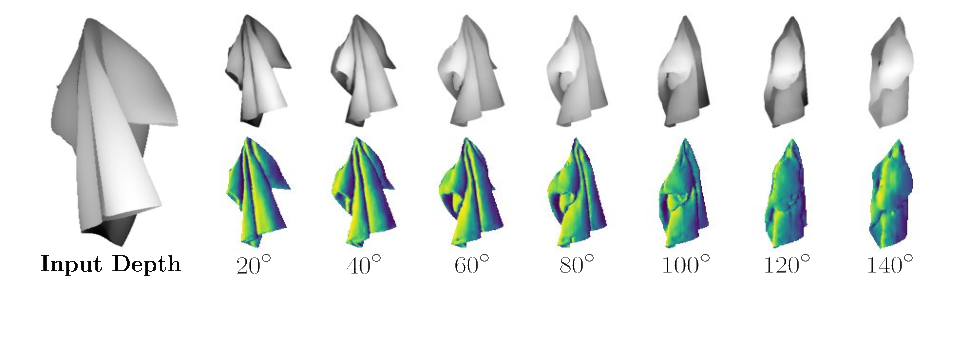
\includegraphics[width=\linewidth]{main/chapter04/data/ipalm_cvpr_image_teaser.pdf}
\end{center}
    \caption[View Synthesis Generation from an input depth map]{\textbf{View Synthesis Generation from an input depth map.} Given a depth map of a deformable cloth (left) and a desired pose defined by a SE(3) rigid transformation, our model generates novel view synthesis preserving the geometry of the input in a high resolution output depth map. In the top row can be seen the depth map estimated by the network while in the bottom is shown the normals map obtained from the predicted depth.}
    \label{fig:teaser}
\end{figure*}

\section{Motivation}

Being able to generate novel depth maps of a deformable cloth under an arbitrary camera view and from a single depth image, can open the door to a number of new exciting applications in different areas, including augmented reality, virtual reality, 3D content production and robotics.

While recent advances in  convolutional neural networks~\cite{varley2017shape, zhou2020learning,haeni2020corn,yan2016perspective} and in particular in those architectures based on the   implicit function~\cite{qiang-nips-2019, chibane20ifnet} have addressed this problem for rigid objects, articulated objects and clothes under mild deformations, there exist no work in doing so for highly deformable and wrinkled clothes, such as the one shown in Fig.~\ref{fig:teaser}. This example corresponds to a T-shirt hanging from a point. Observe that the folds and creases seen from the input depth map rapidly disappear when moving away from the frontal view, while new folds appear. The complexity of this problem also invalidates other geometric approaches that have been used for cloth modelling, like~\cite{salzmann-2010, pumarola2018geometry, golyanik2018hdm, Tsoli_2019_ICCV}, which typically use triangular meshes to represent the underlying shape. In order to keep computational complexity bounded, the resolution of these meshes is quite limited, typically a few tens of vertices, preventing to correctly model complex deformations. 

In this chapter we propose a novel and efficient network to represent depth maps of complex clothing deformations and generating novel views of it. The main novelty of the  network we propose is in its capacity to  perform geometry and occlusion reasoning in the feature space. Concretely, given an input depth map, we initially compute features with an off-the-shelf image encoder-decoder. We then perform projective feature warping according to the desired novel viewpoint we aim to render, and occlusion reasoning, still in the feature domain. We show that these operations, together with an adversarial loss in the spatial domain, allow generating very accurate depth maps, realistically hallucinating the occluded creases and folds.

We train and evaluate  the proposed network on  synthetic and real data, and in both cases we demonstrate its ability to hallucinate unseen and intricate details of deformed cloth. Additionally, the proposed architecture builds upon convolutional blocks, allowing to be executed very efficiently providing the output in a few milliseconds. % This makes our system suitable for motion planning pipeline and control policies for robot textile manipulation.

In summary, our main contributions are the following:
 \begin{itemize}\setlength{\itemsep}{0pt}
\item A novel approach to synthesize depth maps of deformable clothes from arbitrary viewpoints.
\item A novel network that leverages on geometry and occlusion reasoning in the feature space.
%\item A deep model trained from synthetic data and applied to real setup. %\km{feel free to change}
\item A new synthetic dataset of highly deformed cloth with ground truth depth maps. 
\end{itemize}

\section{Related Work}

Inferring multiple viewpoints of an object given an arbitrary image of that object is a highly complex task, especially in the case of non rigid surfaces such as clothes.
Many techniques estimate accurate 3D triangular meshes of deformable surfaces from either single images~\cite{Parashar2019pami,Moreno_pami2013,pumarola2018geometry} (shape-from-template) or video sequences~\cite{Agudo_pami2016,Agudo2017ijcv,Chhatkuli2016cvpr,Moreno_cvpr2011b} (non-rigid shape from motion). These approaches typically rely on the fact that 2D point correspondences between images can be readily established, which is a strong assumption for highly wrinkled and folded clothes. 

Other approaches are more focused on identifying semantically meaningful structures using handcrafted features, to extract generic keypoints~\cite{Simo_ijcv2015}, grasping points~\cite{Ramisa_pr2016,doumanoglou2014active}, wrinkles~\cite{kapusta2019personalized,martinez2017recognition}, edges and corners~\cite{kampouris2016multi}, volumetric features~\cite{li2015folding} and cloth parts~\cite{Ramisa2012using}. Unfortunately, in the case of severe deformed clothes these handcrafted features are not always valid or easy to obtain. For instance, given an arbitrary configuration of a deformed cloth, it could be possible that the semantic features that we are searching for lie in the back side of the cloth, hence, would not be visible and our method would fail.

More recent methods, that are based on neural networks \cite{pumarola2020c,haeni2020corn,xie2019pix2vox} or GANs \cite{HoloGAN2019} try to take advantage of object symmetries to obtain very good view estimations or directly reconstruct a whole object using RGB or depth images \cite{zhou2020learning, yan2016perspective, varley2017shape} or depth \cite{yang-depth-w}. However, these methods assume rigid objects or just minor deformations of non rigid objects \cite{Tsoli_2019_ICCV, golyanik2018hdm}, where a cloth is represented by a low resolution triangular mesh. This is a limited representation for  real life clothes. Many clothes, such as shirts, pants, dresses among others have complicated structures with several seams, that can produce very complex deformations, with strong occlusions. Most of the literature, however, tackle a simplified problem and focus on    reconstructing folds and wrinkles from clothes worn by a human body model \cite{Gundogdu-ICCV-2019, Santesteban-EG-2019, SIZER_Dataset, Patel_2020_CVPR}, which helps to constrain in great measure the type of folds that are formed on the cloth.

These are not the cases we are interested in this chapter, as we aim to reason about cloth objects that are severely deformed. 
For instance, as shown in Fig.~\ref{fig:teaser}, we assume a cloth garment hung from a single point, which generates many wrinkles, folds and self-occlusions. In order to tackle these type of scenarios, we need to go beyond state-of-the-art.

\section{Our approach}
Our framework for estimating the depth of a deformable object from an input depth map and desired rigid transformation is shown in Fig.~\ref{fig_architecture}. We have designed our architecture based on a \textit{Deep Generative Adversarial Neural Network} scheme which intrinsically uses projective geometry theory to reason about the global geometric aspect of the problem. The network is composed of a primary branch, the \textit{Generator}, that regresses the depth map viewed from   a desired pose from which we analytically estimate a normal map and a segmentation mask to separate the object from the background. This principal branch is responsible to learn geometric-aware features using a classic projective geometry pipeline to project learnt features from one view to another. In this same branch, we include another network that combines the original and projected features with and encoding of the applied rigid transformation that is responsible to reason about the potential occlusions and projection order. In addition, we consider a second branch, the \textit{Critic}, that takes the produced depth map and learns to discriminate whether is realistic enough to solve the task and produce more robust solutions to the problem. In the results section we will show that after adapting the projective geometry at the features level, our architecture is able to generate novel synthetic views of deformable cloth depth maps under large camera view changes.


\begin{figure}[!t]
    \centering
    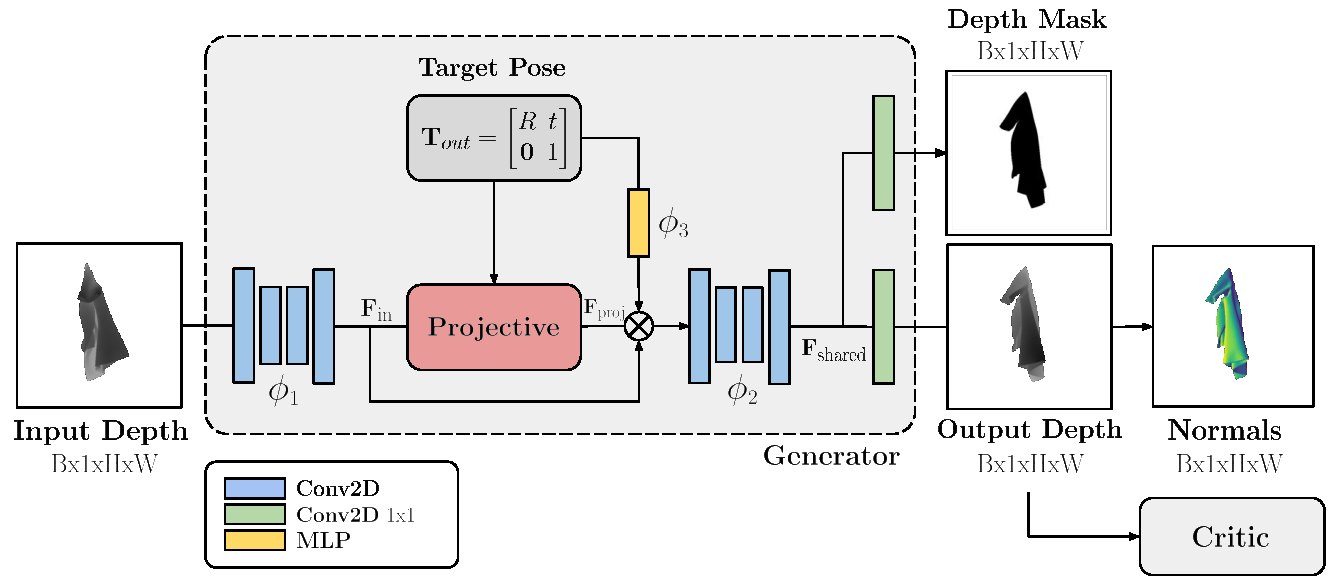
\includegraphics[width=\textwidth]{main/chapter04/data/ipalm_cvpr_architecture.pdf}
    \caption[Proposed architecture for view synthesis generation]{\textbf{Proposed architecture for view synthesis generation.} The proposed architecture consists of two main branches that fulfils in a classic \textit{Deep Generative Adversarial Network} scheme. The first, is the \textit{Generator} that has two prediction heads: foreground/background respect to the object and depth regression from which we perform an analytical estimation of the normals. The second, the \textit{Critic} takes the estimated depth map and classifies as a real or fake sample to help for a better generalisation during the depth regression.}
    \label{fig_architecture}
\end{figure}

%%%%%%%%%%%%%%%%%%%%%%%%%%%%%%%%%%%%%%%%%%%%%%%%%%%%%%%%%%%%%%%%%%%%%%%%%%%%%%%%
%===============================================
\section{Projective Geometry Network}
In this section we give the formulation of the problem that we want to solve and describe the proposed network architecture, which is composed by different components from classical projective geometry. In addition, we also define the different loss functions, including the adversarial training scheme used only during the training of the model.

%===============================================

\subsection{Problem Formulation}
Let $\mathbf{X_w}$ be the 3D world coordinates of a deformed cloth, and $\mathbf{D}_{\textrm{in}} \in \mathbb{R}^{H \times W}$ the depth map representation when seen from a particular perspective defined by a camera pose $\mathbf{T}_{\textrm{w}}^{\textrm{in}}\in$ SE(3) that relates the mapping of the object 3D coordinates from a source camera to a world coordinates system. We aim at designing a \textit{Deep Generative Neural Network} framework that given an input depth map $\mathbf{D}_{\textrm{in}}$ and a desired output pose $\mathbf{T}_{\textrm{w}}^{\textrm{out}}$, synthesizes a new depth map $\mathbf{D}_{\textrm{out}}\in \mathbb{R}^{H \times W}$ by inherently projecting the latent but unavailable $\mathbf{X_w}$ to the desired camera reference frame which can be formally described by the following mapping $(\mathbf{D}_{\textrm{in}}, \mathbf{T}_{\textrm{out}})\rightarrow \mathbf{D}_{\textrm{out}}$.

We assume that the camera calibration parameters are known, namely $\mathbf{K}$ that describes the focal lengths $(f_u, f_v)$, and principal point $(c_u, c_v)$ which are later  used to project the object coordinates from the camera frame to the world coordinate system. Our approach is solved in a supervised manner sampling tuples defined by $\{\mathbf{D}_{\textrm{in}}^i, \mathbf{T}_{\textrm{out}}^i, \mathbf{D}_{\textrm{out}}^i\}_{i=1}^N$ from the dataset used both for training and evaluation (different splits). With our method we do not intend to do an explicit reconstruction of the object shape, but instead learn geometric invariant features through a process of features projection from one view to another for later combining and reason about the occlusions.

\subsection{Network architecture}
Given an input depth image $\mathbf{D}_{\textrm{in}}$, of size $H\times W$, the initial step consists in extracting a set of dense local features per pixel. Following~\cite{pix2pix2017} we feed $\mathbf{D}_{\textrm{in}}$ into a first encoder-decoder network which is configured in such  a way that the bottleneck has  small downsampling factor of 2. Let us denote these features as $\phi_1(\mathbf{D}_{\textrm{in}}) \rightarrow \mathbf{F}_{\textrm{in}}$ of size $F\times H \times W$. The intuition is that these local features will keep information of the 3D local structures in order to later reason about the depth ordering to perform the view projection.

\vspace{1mm}
\noindent{\textbf{Projective features warping}}. In order to make the features robust to viewpoint changes, we have designed a differential operator that using simple projective geometry warps the learnt features $\mathbf{F}_{\textrm{in}}$ to the desired output pose $\mathbf{T}_{\textrm{w}}^{\textrm{out}}$. The operator assumes to have a calibrated setup, which using the following equation:
\begin{equation}
    \mathbf{H}_{\textrm{in}}^{\textrm{out}} = \mathbf{K} \cdot \mathbf{T}_{\textrm{w}}^{\textrm{out}} \cdot (\mathbf{T}_{\textrm{w}}^{\textrm{in}})^{\textrm{-1}} \cdot \mathbf{K}^{\textrm{-1}}
\end{equation}
This expression will give us the transformation to project features from one view to the desired output pose. Following a similar approach as in~\cite{NIPS2015_5854, eriba2020kornia} we can later perform a differentiable bilinear sampling such that:
 \begin{equation}
    \omega(\mathbf{F}_{\textrm{in}}, \mathbf{H}_{\textrm{in}}^{\textrm{out}}, \mathbf{D}_{\textrm{in}}) \rightarrow \mathbf{F}_{\textrm{proj}}
 \end{equation}
That is, projects $\mathbf{F}_{\textrm{in}}$ according to $\mathbf{H}_{\textrm{in}}^{\textrm{out}}$, obtaining $\mathbf{F}_{\textrm{proj}}$. This operator will produce a stack of features of size $F\times H \times W$ that will help later the system to be invariant to viewpoint changes.

\vspace{1mm}
\noindent{\textbf{Occlusion comprehension}}. One of the challenges for our method is the way occlusions are solved when we project features between two different views. Initially, our system assumes no knowledge about the explicit shape of the object, in the  sense that during the features projection there is no notion about the depth ordering,  or in other terms, what is front or behind. Since we want to let our system to reason about how to handle occlusions, we will take the original and warped features along with an embedding of the desired pose and feed  them to a second network:
\begin{equation}
    \phi_2(\mathbf{F}_{\textrm{in}}, \mathbf{F}_{\textrm{proj}}, \phi_3(\mathbf{T}_{\textrm{in}}^{\textrm{out}})) \rightarrow \mathbf{F}_{\textrm{shared}}
\end{equation}
This expression generates $\mathbf{F}_{\textrm{shared}}$, which will encode the combined information from the input depth map and its projection. We denote this second network as an auto-encoder with a downsampling factor of $8$. A large factor, will force the network to have also a large receptive field so that the captured information comes from the whole scene and make easy to resolve the occluded information.

\vspace{1mm}
\noindent{\textbf{Task aware prediction.}} Our system has a pre-final step where $\mathbf{F}_{\textrm{shared}}$ is fed to the two different network heads. The final heads of the network are small learnt kernels of $1\textrm{x}1$ that will specialise for each of the sub-tasks. The first, produces $\mathbf{D}_{\textrm{out}}$ with the actual regression values of the depth map and from which using analytical methods, we estimate the normal maps. Finally, the second head produces $\mathbf{D}_{\textrm{mask}}$ that represents a segmentation mask of foreground and background of the object respect to the scene.


\vspace{1mm}
\noindent{\textbf{Depth critic.}} In our method we implement a critic network $D$ as in PatchGan~\cite{isola2018imagetoimage} that maps from an input depth map to a matrix $\mathbf{Y}_{I} \in \mathbb{R}^{26\text{x}26}$, where $\mathbf{Y}_I[i,j]$ represents a probability for each patch overlapping $ij$ to be a real sample. This critic network enforces high frequency correctness in order to reduce the blurriness of the generated depth maps and make them more close to the ones from the training distribution.

\subsection{Loss functions}

The training of our model is a composition of losses that tries to enforce different aspects of the cloth configuration and preserve implicit consistency on the 3D shape. As described in the previous section, our architecture has two different output heads, the first to predict a depth map and the second a mask. We next describe in detail the different losses used for optimising the model parameters:

\vspace{1mm}
\noindent{\textbf{Weighted depth regression loss.}} The main loss function for our model optimises the depth pixels values produced by our model with respect to the ground truth data. We define this cost function in terms of a weighted \textit{Mean Square Error} that will be evaluated on the foreground object:

\begin{equation}
     L_\textrm{D} = \frac{1}{n}\sum_{t} \lambda_t \cdot \| \mathbf{D}_{\textrm{out}}(t) - \mathbf{D}_{\textrm{GT}}(t) \| _2 ^ 2\;,
\end{equation}
where $\mathbf{D}_{\textrm{GT}}$ is the ground truth depth map and $n$ are the number of foreground pixels $t$, i.e. pixels with a depth value. We define $\lambda_t$ as weighting term which is computed by projecting the original input depth map $\mathbf{D}_{\textrm{in}}$ to produce a coarse depth map $\mathbf{D}_{\textrm{coarse}}$ and compare against $\mathbf{D}_{\textrm{GT}}$ to obtain a mask of the occluded regions. $\lambda_t$ can be seen as an attention mechanism during the training to make the model to optimise better the parts of the cloth with missing or occluded information.

\vspace{1mm}
\noindent{\textbf{Binary mask loss.}} The second loss we consider is a binary classification loss function which accounts for the number of valid pixels in the output depth image. This loss is defined in terms of a {\em Cross Entropy} using the depth values to the infinity to define the ground truth mask:
\begin{equation}
     L_\textrm{M} = - \frac{1}{n} \sum_{t} \mathbf{D}_{\text{mask}}(t) \cdot \log(\hat{\mathbf{D}}_{\text{mask}}(t))
\end{equation}
where $\hat{\mathbf{D}}_{\text{mask}}$ is the ground truth for the valid depth map, and $n$ the total number of foreground pixels $t$ in the depth images.

\vspace{1mm}
\noindent{\textbf{Depth gradients regularisation.}} Predicting the folds in the cloth is a difficult task for the network without an extra supervision. For this reason, we add an extra term loss that will try to constrain the network to preserve the predicted gradients on the depth image with respect to the ground truth. This loss is computed as follows:
\begin{equation}
    L_\textrm{S} = {\mid \text{\textit{Sobel}}(\mathbf{D}_{\textrm{out}}) - \text{\textit{Sobel}}(\mathbf{D}_{\textrm{GT}}) \mid}
\end{equation}
where $\text{\textit{Sobel}}$ is a differentiable Sobel edge operator~\cite{eriba2020kornia} that computes the normalised edge image gradients within the depth domain.

\vspace{1mm}
\noindent{\textbf{Normal maps regularisation.}} We want our method to be robust under geometric transformations. Similar to the depth gradients regularisation method, we force our loss function to optimise the normal maps computed from the output depth map $\mathbf{D}_{\textrm{out}}$. Our final loss function, contains an extra term so that the computed normals from the predicted depth are forced to be close from the ground truth ones. The normal loss can be written in terms of a cosine similarity:
\begin{equation}
        L_\textrm{N} = \frac{1}{n} \sum_{t} \dfrac{\mathbf{N}_{\textrm{out}}(t) \cdot \mathbf{N}_{\textrm{GT}}(t)}{\max(\Vert \mathbf{N}_{\textrm{out}}(t) \Vert _2 \cdot \Vert \mathbf{N}_{\textrm{GT}}(t) \Vert _2, \epsilon)}\;,
\end{equation}
where $\mathbf{N}_{\textrm{out}}$ and $\mathbf{N}_{\textrm{GT}}$ are the Normal maps computed from the depth map prediction and ground truth, respectively. $\epsilon$ is a small value to prevent division by zero, and again, $n$ are the number of foreground pixels $t$. In order to compute the normal maps, we  use a differentiable operator~\cite{eriba2019kornia, eriba2020kornia} that using the camera calibration matrix (referred as $\textbf{K}$), maps the depth map to a point cloud and from neighbour points computes the 3D spatial gradients. Then, we can compute an approximation of the normal maps with the cross product of the derivatives at each 3D point.

\vspace{1mm}
\noindent{\textbf{Adversarial loss.}} In order to optimize our main network branch, namely the generator $G$, and force it to produce depth maps that follow the same distribution as the training data, we use a modified version of the standard GAN algorithm~\cite{NIPS2014_5ca3e9b1} proposed by WGAN-GP~\cite{NIPS2017_892c3b1c}. Specifically, the original GAN formulation is based on the Jensen-Shannon (JS) divergence loss function and follows a \textit{min-max strategy game} between the generator $G$ and the critic $D$. The last tries to correctly classify real and fake depth images while the generator will try to foul the critic. This loss is extremely unstable and not continuous with respect to the parameters coming from the generator and can easily saturate the system leading to vanishing gradients in the critic. This issue is solved in WGAN~\cite{arjovsky2017wasserstein} which proposes to replace the JS with the continuous Earth Mover Distance. In order to maintain the Lipschitz constraint, WGAN-GP~\cite{NIPS2017_892c3b1c} proposes to add a penalty term for the critic network computed as the norm of the gradients with respect to the critic input. In our work we formulate the loss as follows:
\begin{align}
    L_\textrm{A} & = \mathbb{E}_{\textbf{I} \sim \mathbb{P}_o}[D(G(\mathbf{D}_{\textrm{in}}))] - \mathbb{E}_{\textbf{I} \sim \mathbb{P}_o}[D(\mathbf{D}_{\textrm{out}})] + \lambda_{gp} \mathbb{E}_{\tilde{\mathbf{I}} \sim \mathbb{P}_{\tilde{\mathbf{I}}}}[(|| \nabla_{\tilde{I}} D(\tilde{I}) ||_2 - 1) ^ 2]
\end{align}
where $\lambda_{gp}$ is a penalty coefficient.

\vspace{1mm}
\noindent{\textbf{Total loss.}} Our final loss is the average of the different losses described before:
\begin{equation}
     \text{Loss} =\frac{1}{5}(L_{\textrm{D}} + L_{\textrm{M}} + L_{\textrm{S}} + L_{\textrm{N}} + L_{\textrm{A}}) 
\end{equation}

\section{Experimental setup}

\begin{figure}
    \centering
    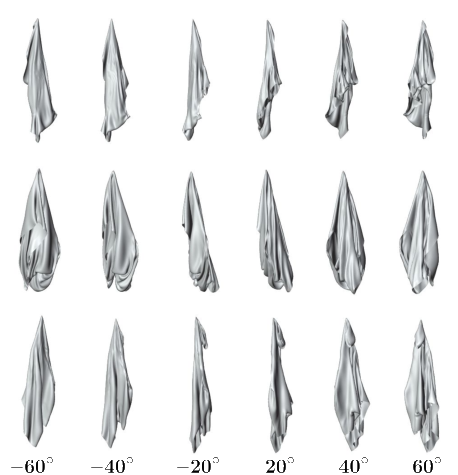
\includegraphics[width=\linewidth]{main/chapter04/data/ipalm_cvpr_grid_dataset_synth.pdf}
    \caption[Sample images of the synthetic dataset]{{\bf Sample images of the synthetic dataset.} We build a large dataset of deforming clothes viewed by a ring of 36 depth cameras. The cloth model is hung from a different position (rows) and captured from several cameras (columns).}
    \label{fig_setup_cameras}
\end{figure}

The model is trained with a synthetically generated dataset, using depth images of size $H \times W = 512 \times 512$. The image features $\phi_1$ and $\phi_2$ are obtained from an auto-encoder with skipped connections~\cite{pix2pix2017} and a downscaling factor of 2 and 8, respectively. The resulting feature maps from $\phi_1(\mathbf{D}_{\textrm{in}})$ are of size of $F\times H \times W = 32 \times 512 \times 512$.% Additionally, we normalize the depth maps by its mean and standard deviation, and the input depth map background mask is concatenated to the input of $\phi_1$.
The computed embedding for $\phi_3(\mathbf{T}_{\textrm{in}}^{\textrm{out}})$ has also size of 32, which is later expanded and concatenated to every pixel of $\mathbf{F}_{\textrm{in}}$ and $\mathbf{F}_{\textrm{out}}$. The head for predicting the output depth map $\mathbf{D}_{\textrm{out}}$ has a non-linearity \text{TanH} to keep the distribution normalized. We use Adam solver~\cite{kingma2017adam} with a learning rate of 0.0001 for both the generator and discriminator, $\beta1 = 0$ , $\beta2 = 0.999$ and a Cosine Annealing learning rate scheduling~\cite{LoshchilovH16a}.  The model is trained with a batch size of 8 in a single Nvidia\textsuperscript{\textregistered} GTX 1080 for 1 day.

\section{Experimental Results}
To evaluate the proposed method, we experiment with both synthetic and real datasets. In the following, we first describe our configuration of the two datasets, then explain in detail the training strategy, and finally provide both quantitative and qualitative results.

\subsection{Dataset}

\vspace{1mm}
\noindent{\textbf{Synthetic data generation.}} We show in Fig.~\ref{fig_setup_cameras} three different examples of the sequences (sampled at 20$\deg$) we produce using the physics cloth engine of Blender~\cite{Blender}. The setup for generating these depth maps consists in a deformed t-shirt model surrounded by a rig of $36$ cameras in a circle separated by steps of $10$ degrees. Specifically, the bounding box defined by the deformed mesh lies at the center of the circle, and we set the radius to $120$cm to ensure the whole t-shirt mesh is completely visible by all cameras.

A 3D human body design suite~\cite{Makehuman} is used to obtain the t-shirt model. This model is defined by a quad mesh with $3.500$ vertices, which is the best topology for the cloth physics engine simulator. The cloth physics engine is based on a spring mass model, which contains several cloth fabric presets as well as several parameters that are tunable for adjusting the behaviour of the simulation. We use the \textit{cotton} preset in the case of the t-shirt, and just modify the bending and stiffness parameters to achieve more realistic deformations. The t-shirt mesh is hung from  a point and let deform by gravity. The deformation process is run for $250$ steps on each physics simulation to ensure a rest position is achieved. Before running each simulation, the mesh is randomly rotated, and a vertex is also randomly chosen as a hanging point. 

The complete dataset consists of $1.000$ simulations and for each simulation  the depth image, normal image, background segmentation, and intrinsic and extrinsic camera matrices are recorded. We pick $100$  simulations for training the network, $30$ for validation and $30$ for test. There is no overlap between the three splits.

\vspace{1mm}
\noindent{\textbf{Real data generation.}} A t-shirt is grasped by a Baxter robot and naturally hung under gravity. 
We manually adjusted real-world setup to roughly match the appearance and dynamics of the simulation. Specifically, an Intel RealSense L515 camera is placed $120$cm away from the grasping point. The robot continuously rotates the t-shirt while depth images are captured in the meanwhile.

The whole real dataset consists of 100 sequences, with 36 depth images (every 10 rotation degree) in each sequence. 
The clothes are grasped from different points in different sequences. The entire acquisition process takes approximately 16 hours. We segment the garment from the background by thresholding the depth between $110$cm and $130$cm. Then, the acquired depth images are cropped to remove the non-garment parts of the image and resized to $512\times512$ pixels.
We use $50$ out of 100 sequences for training the network, $15$ for validation and $15$ for test.


\subsection{Incremental training}

During the study to determine the maximum rotation angle by our system we found that training our model from scratch does not converge to an optimal solution. We experimentally found that the best approach to tackle this problem is using the so well known \textit{Curriculum Learning} training technique and train our system in a incremental manner starting with "easy" data samples and increase the complexity of the task by showing to our model more "difficult" samples with coming views with larger angle rotations.

The process we adopt to sample our training data is as follows: First, a subset of simulations is randomly sampled from the total number of  simulations in the dataset. Second, we randomly pick two depth maps for each of the simulation, one shall be the input depth map $\mathbf{D}_{\textrm{in}}$ and the other the output $\mathbf{D}_{\textrm{out}}$. We will also annotate the training sample with  the rotational angle between the two depth maps.

To train the network, we need several interactions. To be more specific, in the first iteration, we sample source and destination depth which are are most 10 degrees apart.  The network is trained until converge and ensuring a validation loss below a certain threshold.  Then, in the next iteration, we increase the training dataset by including more samples from rotations up to 20 degrees, and we start the training again initialising the weights with the ones obtained from the previous stage. We repeat this incremental process for 40, 60, 80 ... 180 degrees. We observed that by following this training procedure we can obtain a faster training convergence for large rotation angles.   

\begin{figure}
    \centering
    \begin{tabular}{cc}
    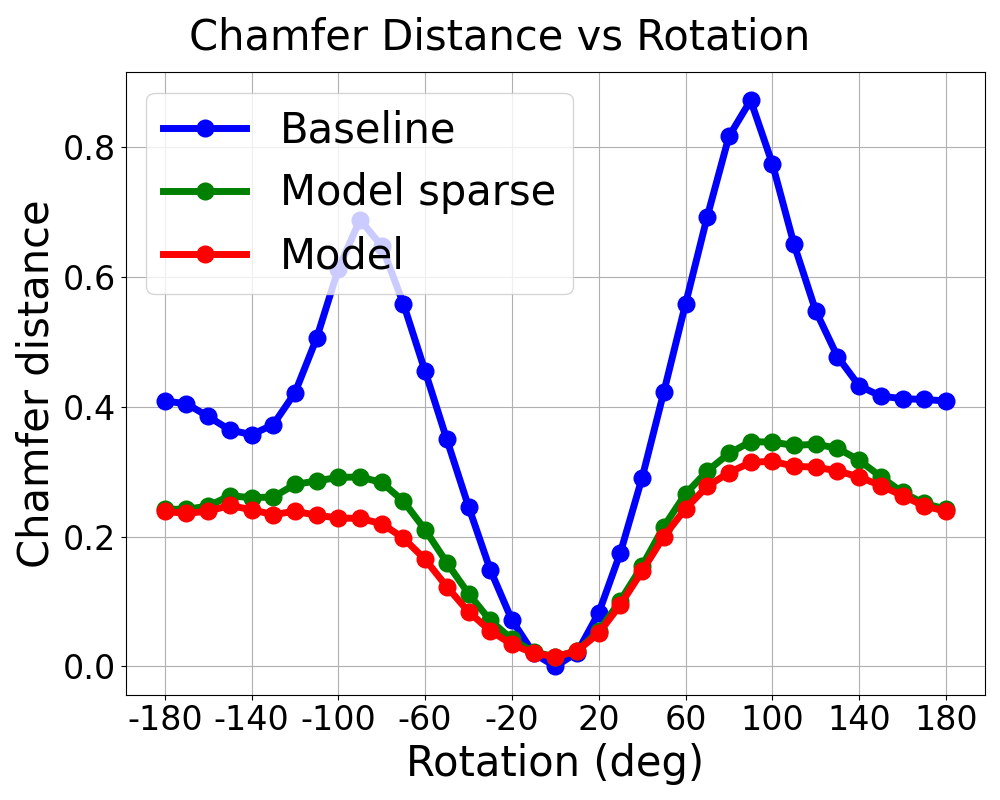
\includegraphics[scale=0.2]{main/chapter04/data/plot_chamfer_synth.png} &
    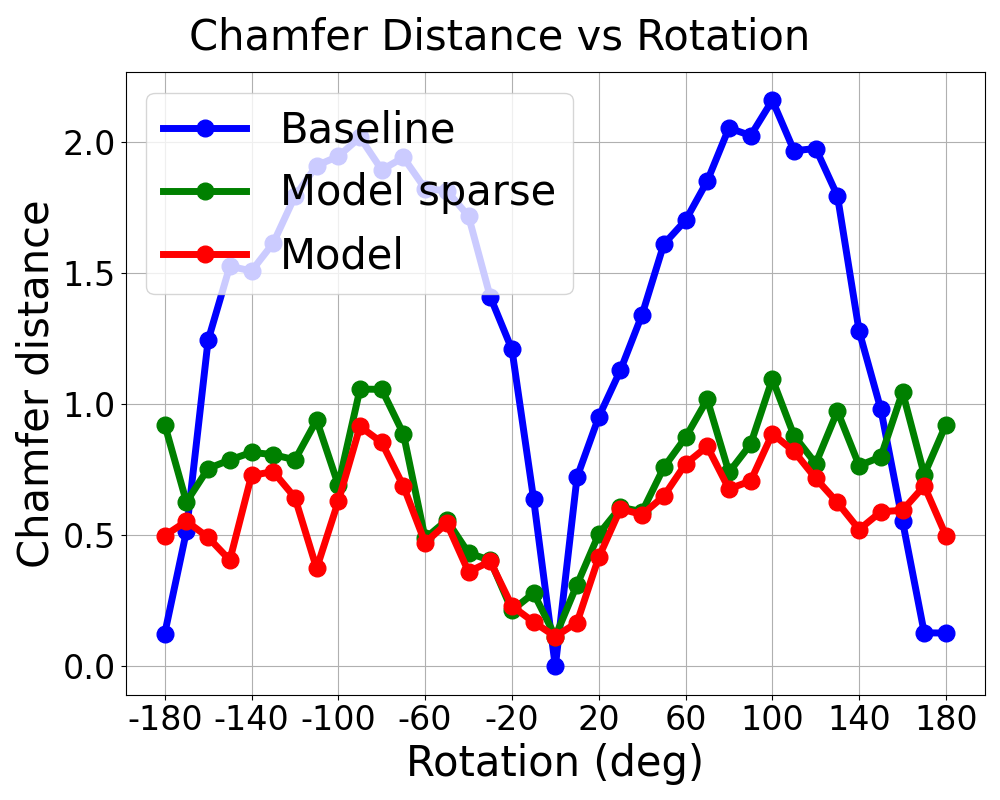
\includegraphics[scale=0.2]{main/chapter04/data/plot_chamfer_real.png}\\
    \end{tabular}
    \caption[Evaluation on synthetic and real data for the Chamfer distance]{{\bf Evaluation on synthetic and real data for the Chamfer distance.} Evaluation of the network performance when generating novel views from the same input depth map under different rotation angles. {\em Baseline} is the analytic geometric rotation of the input depth map. {\em Model} is the result obtained from our network. {\em Model sparse} is the result of the proposed model, evaluated only on the image pixels that have a valid depth after the projection between the two views. Chamfer distance vs the rotation for synthetic (left) and real (right) data. The lower the better.}
    \label{fig_plot_synth_rotations_chamfer}
\end{figure}

\def\rot#1{\rotatebox{90}{#1}}
\begin{figure}
    \centering
    \begin{tabular}{cccc}
    \rot{~~~~~\textbf{Synthetic}} &
    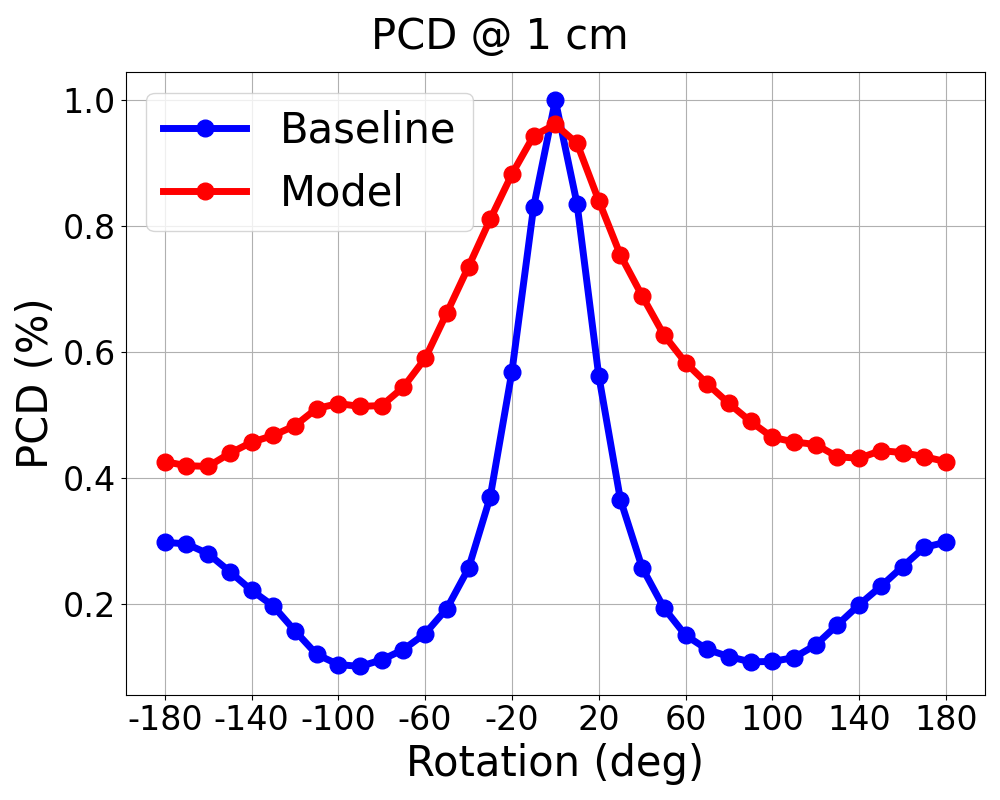
\includegraphics[scale=0.13]{main/chapter04/data/plot_pcd_1_synth.png} &
    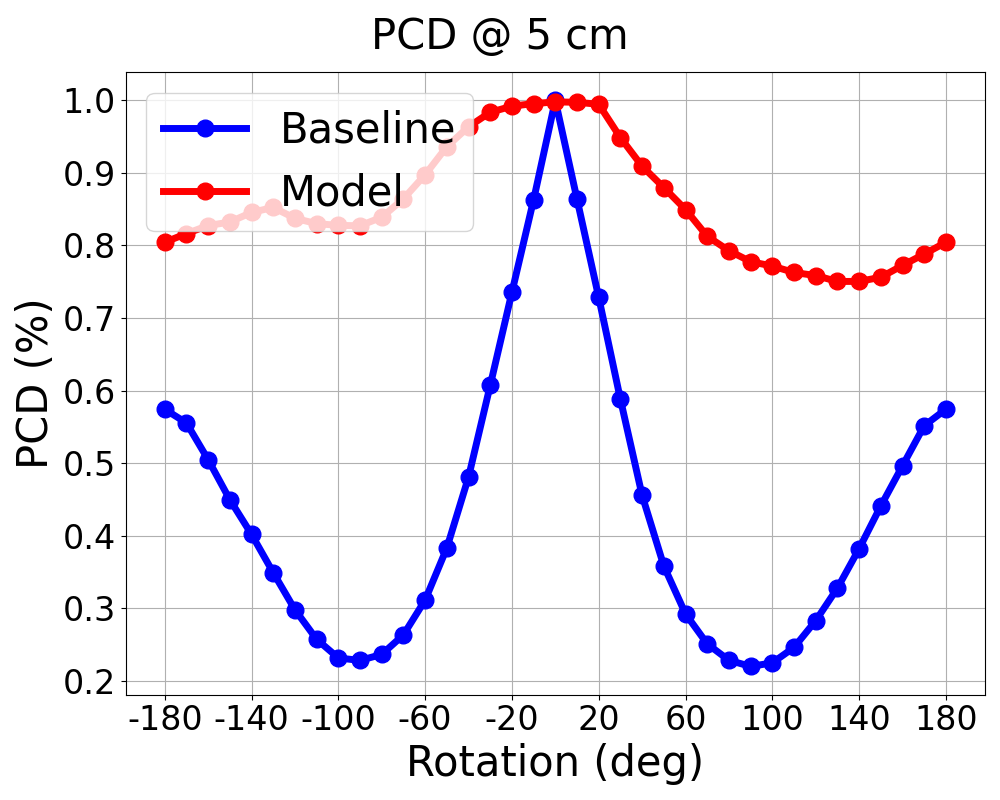
\includegraphics[scale=0.13]{main/chapter04/data/plot_pcd_5_synth.png} &
    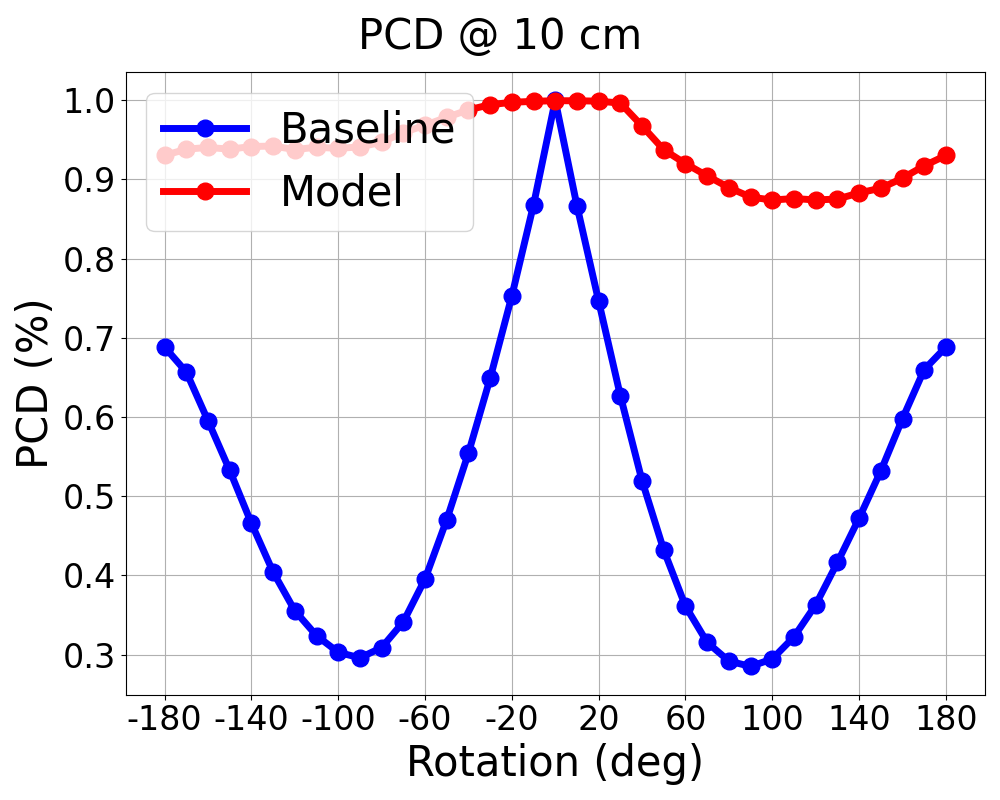
\includegraphics[scale=0.13]{main/chapter04/data/plot_pcd_10_synth.png}\\
    \rot{~~~~~~~~~~\textbf{Real}} &
    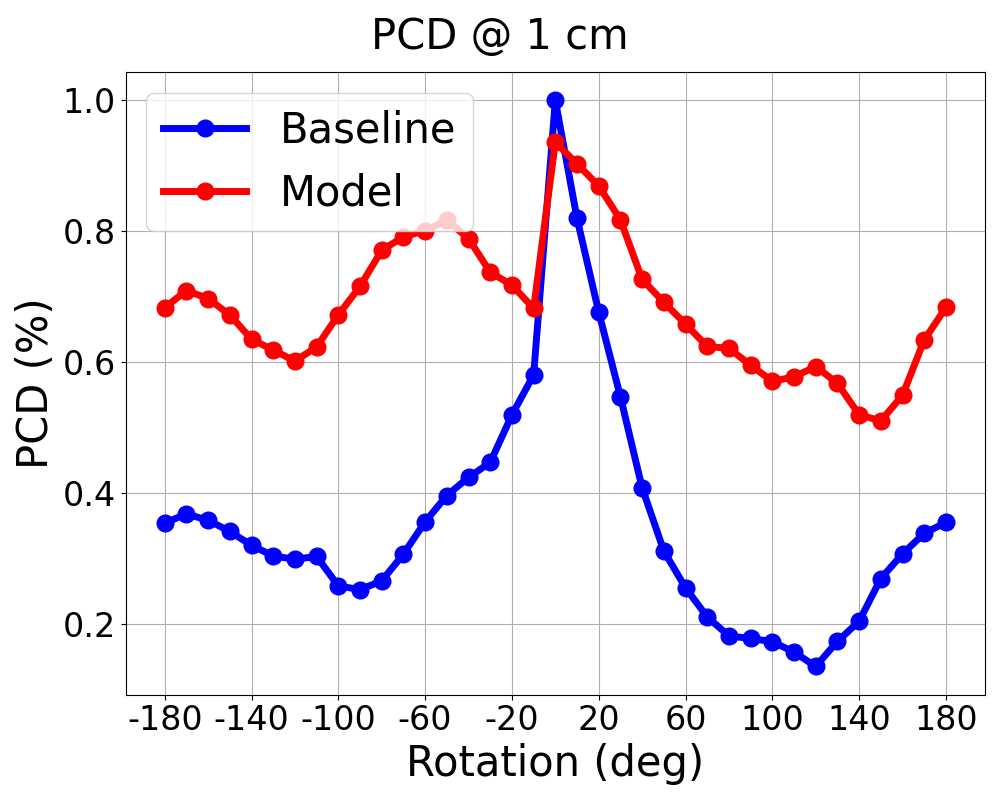
\includegraphics[scale=0.13]{main/chapter04/data/plot_pcd_1_real} &
    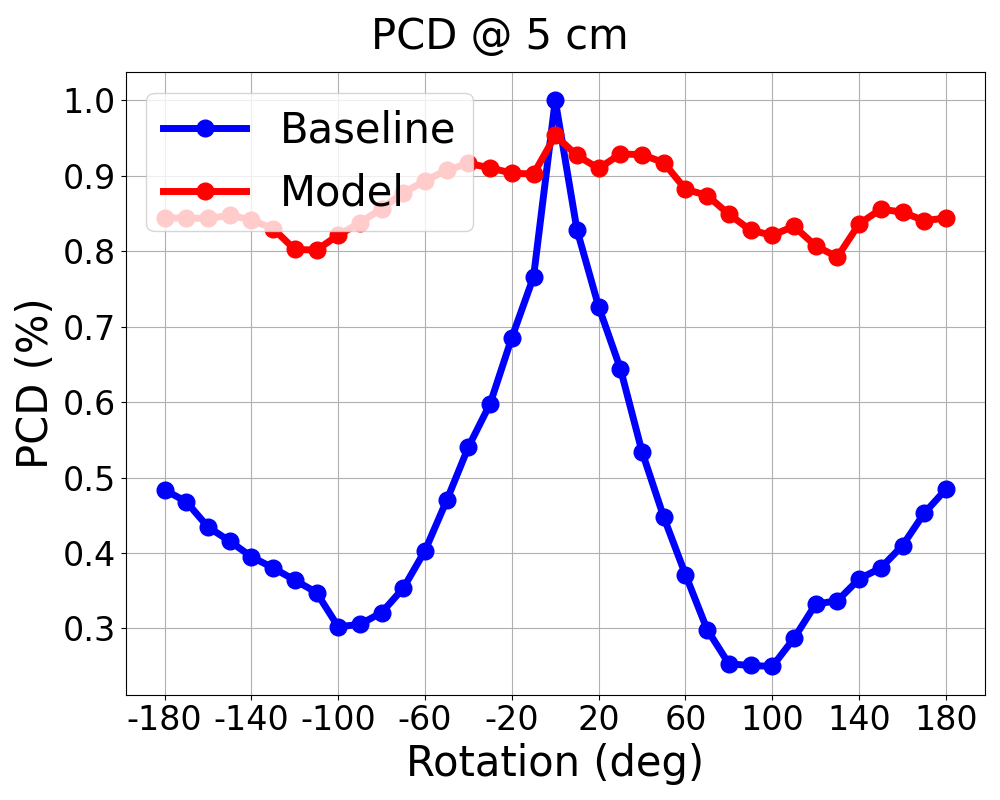
\includegraphics[scale=0.13]{main/chapter04/data/plot_pcd_5_real} &
    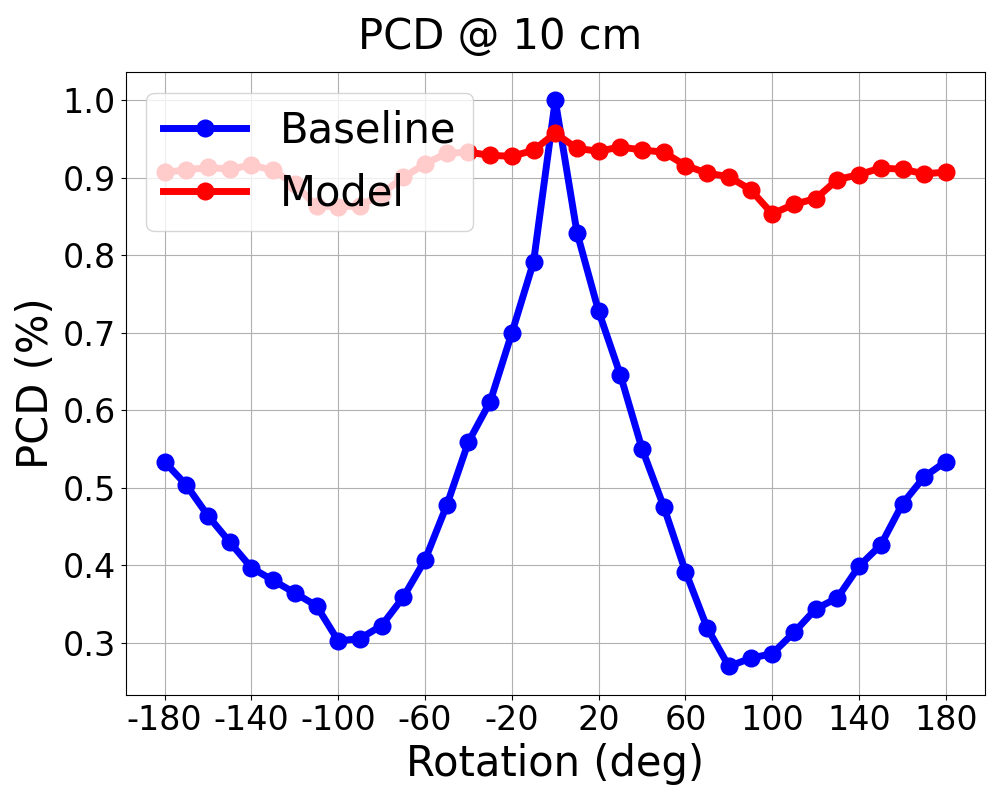
\includegraphics[scale=0.13]{main/chapter04/data/plot_pcd_10_real}\\
    \end{tabular}
    \caption[Evaluation on synthetic and real data for the Percentage Correct Depth]{{\bf Evaluation on synthetic and real data for the Percentage Correct Depth.} Similar to the figure~\ref{fig_plot_synth_rotations_chamfer}, we show the performance of our network in terms of Percentage Correct Depth (PCD) at different accuracy: [1, 5, 10] cm. The higher the better.}
    \label{fig_plot_synth_rotations_pcd}
\end{figure}

\subsection{Quantitative Evaluation}

We next evaluate the accuracy of our trained model under different rotation angles using both the  synthetically generated and real datasets. In order to perform the evaluation, we compare against {\em Baseline} which is  a coarse depth map obtained by analytically rotating the 3D points of the input depth map to the desired view.

We report the evaluation on the synthetic data using the best performing model. The model has been trained using up to  180 degrees of rotation following the described \textit{Curriculum Learning} approach. For the real data, we have taken the model trained on the synthetic dataset and finetuned using the real training data.

\newcommand{\bgt}{\bD_{\textrm{GT}}}
\newcommand{\bdcoarse}{\bD_{\textrm{coarse}}}

In order to report the evaluation, we use two different metrics: the bidirectional \textit{Chamfer Distance} and the \textit{Percentage of Correct Depth (PCD)}, which are defined as follows. 

Let $\mathbf{\hat{D}}$ be the estimated depth map and $\mathbf{D}_{\textrm{GT}}$ the ground truth depth map. The bidirectional Chamfer Distance is computed as follows:
\begin{equation}
\begin{small}
\textrm{Chamfer}(\mathbf{\hat{D}}, \mathbf{D}_{\textrm{GT}})=\frac{1}{2}(\textrm{KNN}(\mathbf{\hat{D}} \rightarrow \mathbf{D}_{\textrm{GT}})+ \textrm{KNN}(\mathbf{D}_{\textrm{GT}} \rightarrow \mathbf{\hat{D}}))
\end{small}
\end{equation}
where $\textrm{KNN}(\mathbf{\hat{D}} \rightarrow \mathbf{D}_{\textrm{GT}})$ represents the average Euclidean distance for all points of $\mathbf{\hat{D}}$ to their nearest neighbor in $\mathbf{D}_{\textrm{GT}}$. Note that $\textrm{KNN}(\cdot ,\cdot)$ is not a true distance measure because it is not symmetric. This is why we compute it bidirectionally. 

We also asses the accuracy of our method under different error thresholds using the {\em Percentage of Correct Depth (PCD)}, which represents the percentage of predicted depth pixels with a depth error below a certain threshold. For instance, PCD@k represents the per- centage of predicted depth pixels with a depth error below k. 

In Fig.~\ref{fig_plot_synth_rotations_chamfer} and~\ref{fig_plot_synth_rotations_pcd} we report the described error metrics for both the synthetic and real data experiments. As can be appreciated, our method is able to generate results with a higher accuracy compared to the baseline in all the rotation angles. In the first column experiments we demonstrate that how our model is always below the baseline in terms of the Chamfer Distance error. In this particular case, we also report the error of ``Model sparse'', in which the error is only evaluated on the $(u,v)$ pixels of the depth image for which the baseline has valid depth values after the projection from the original view. The  reported error for ``Model sparse'', is very similar to the full model performance, which indicates that the model is able to correctly predict both the already seen points, as those that needs to hallucinate. 

When considering the PCD metric, our model also consistently imporved the baseline. It is  worth noticing that for our model PCD$@$5cm surpasses always 0.8, that is, at least $80\%$ of the estimated depth points have an error of 5cm or less. The magnitude of this error would give to us enough precision to use the method in some the applications mentioned before such as augmented or virtual reality.

Fig.~\ref{fig_outputs_synthetic} and~\ref{fig_outputs_real} show visual results of the generated data using our best performing model under a range  of $[-180,180]$ degrees of rotation. Note that for large rotations ($\pm 180$ degrees) the baseline is affected by gross errors and displays erroneous folds. Our approach, although a bit blurry, is able to recover the main structures of folds and creases.

\begin{figure}[!h]
\begin{center}
    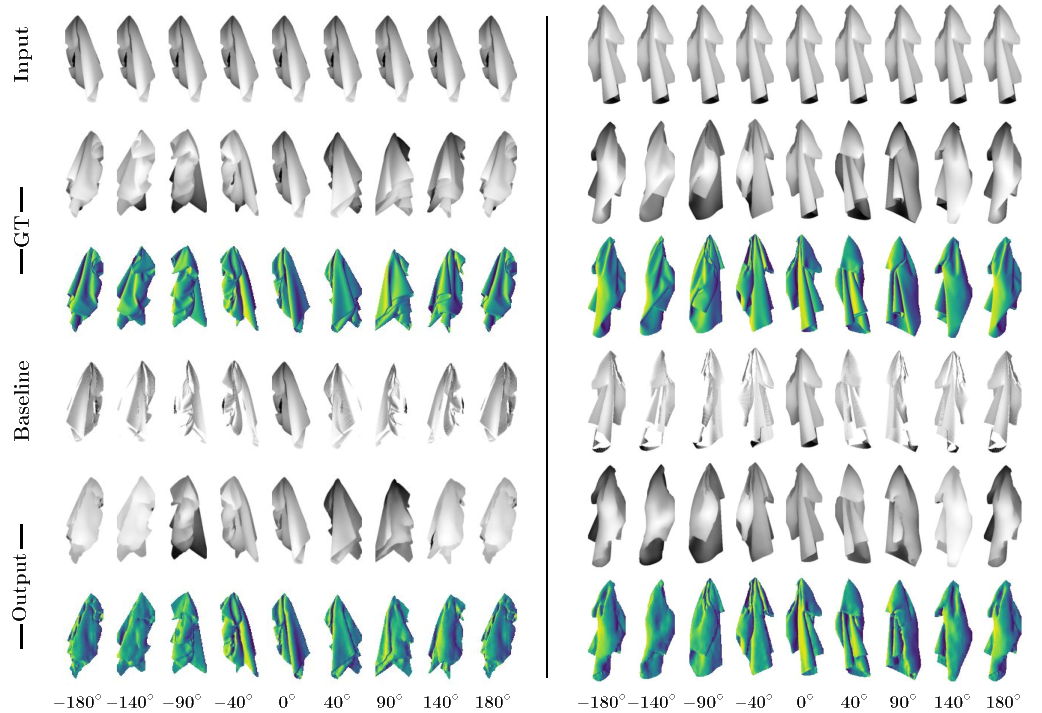
\includegraphics[width=\linewidth]{main/chapter04/data/ipalm_cvpr_grid_synth_vertical.pdf}
    \caption[Qualitative results on synthetic data]{{\bf Qualitative results on synthetic data.} Outputs produced by our model under two different simulations (Left to Right blocks) showing several rotations from -180 to 180 degrees in the Z-axis (Left to Right columns). \textbf{Row 1:} Input depth map used to hallucinate the novel views. \textbf{Row 2-3:} Ground truth depth and normals maps from the evaluation set. \textbf{Row 4:} Baseline computed from the input depth map. \textbf{Row 5-6:} Predicted Depth map and the normals computed analytically from the predicted Depth.}
    \label{fig_outputs_synthetic}
\end{center}
\end{figure}

\begin{figure}[!h]
\begin{center}
    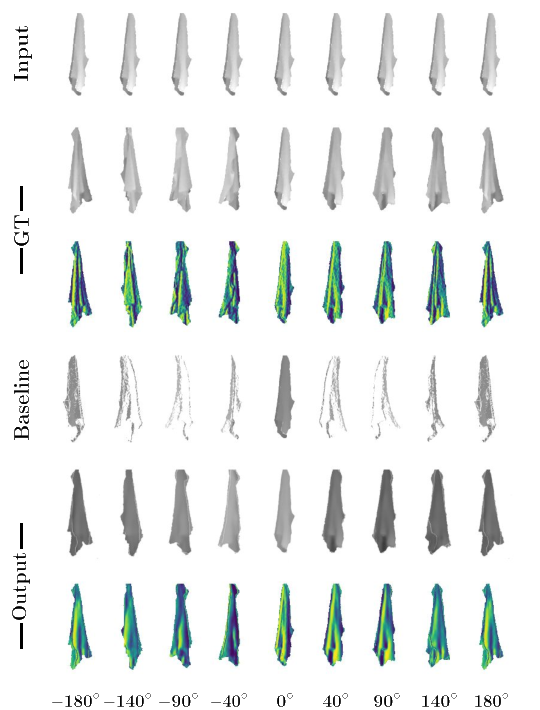
\includegraphics[width=0.5\linewidth]{main/chapter04/data/ipalm_cvpr_grid_real_vertical.pdf}
    \caption[Qualitative results on real data]{{\bf Qualitative results on real data.} Results obtained with our network on a sequence captured from a real camera setup. Similar to Figure.~\ref{fig_outputs_synthetic}, the network produce new views from different rotation in the Z-axis from -180 to 180 degrees. \textbf{Row 1:} Input depth map. \textbf{Row 2-3:} Ground truth depth and normals maps. \textbf{Row 4:} Baseline computed from the input depth map. \textbf{Row 5-6:} Predicted Depth map and the normals computed analytically from the predicted Depth.}
    \label{fig_outputs_real}
\end{center}
\end{figure}

\subsection{Ablation study}

In the following we evaluate the performance of the network under different configurations (with and without the adversarial loss). The study, similar to the experiments discussed in Figure~\ref{fig_plot_synth_rotations_chamfer} reports the \textit{Chamfer distance} metric  between ground truth and estimated point clouds  and the \textit{Cosine Distance} between normal maps.  For further comparison, we also include the performance of the model {\em Baseline}. As observed in the Table~\ref{table_ablation_study}, the use of the GAN loss brings certain improvement both in the real and synthetic experiments. Our model, with and without GAN, significantly improves the Baseline.

\begin{table}[!tbh]
\begin{center}
\resizebox{\textwidth}{!}{
\begin{tabular}{lcccc}
\toprule
& \multicolumn{2}{c}{Synthetic Data} & \multicolumn{2}{c}{Real Data} \\
Method & Chamfer$\downarrow$ & Cosine$\downarrow$ & Chamfer$\downarrow$ & Cosine$\downarrow$ \\
\cmidrule(lr){1-1}  \cmidrule(lr){2-3} \cmidrule(lr){4-5}
Baseline  
& 0.2147 $\pm$ 0.11  
&  -
&   1.4500 $\pm$ 0.56     
&  - \\

Network w/o GAN
& 0.0568 $\pm$ 0.02     
& 0.8320
& 2.0092 $\pm$ 0.23        
& 0.6528 \\ 

Network with GAN
& 0.0348 $\pm$ 0.01     
&  0.8314
& 0.5530 $\pm$ 0.17
& 0.6216 \\ 
\bottomrule
\end{tabular}
}
\caption[Quantitative results under different network configurations]{{\bf Quantitative results under different network configurations.} The table shows the results in terms of \textit{Chamfer distance}   mean and standard deviation and the \textit{Cosine Distance}  between the normals maps for the Baseline and the model trained with and without the Adversarial loss. The evaluation has been done from -180 to 180 degrees of rotation.}
\label{table_ablation_study}
\end{center}
\end{table}

\section{Conclusions}

In this chapter we have proposed an approach to synthesize novel views of depth maps for deforming clothes. We have shown that encoding the input depth map using spatial-aware features, and geometrically transforming these features, allows hallucinating complex details, like folds and creases, which were not visible in the input depth map. Moreover, we have shown that our method is capable to recuperate many details in very extreme viewpoints where the geometric information is very little, since it is lost by the self-occlusions.
We have presented several quantitative results on a synthetic dataset and proof that the proposed method also can work with real data captured by a depth sensor. Finally, the system is based on purely convolutional blocks, allowing to perform inference in a few milliseconds and uses the library proposed in chapter~\ref{chap:chap_03} to include classical projective geometry techniques within the computational graph.